\question [20] No triângulo retângulo isósceles XYZ conforme desenho abaixo, em que XZ = YZ = \SI{3,0}{\centi\meter}, foram colocadas uma carga elétrica puntiforme $Q_x=\SI{+6}{\nano\coulomb}$ no vértice   e uma carga elétrica puntiforme $Q_x=\SI{+8}{\nano\coulomb}$ no vértice Y. A intensidade do campo elétrico resultante em Z devido às cargas já citadas é? \\
	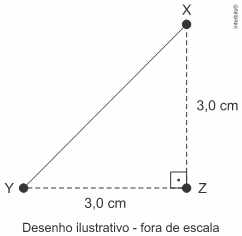
\includegraphics[width=0.3\linewidth]{questoes/imagens/q5}\\
	(Dados: o meio é o vácuo e a constante eletrostática do vácuo é $k=\SI[per-mode = symbol]{9e9}{\newton\meter\tothe{2}\per\coulomb\tothe{2}}$)  

		\begin{EnvUplevel}

			\begin{choices}
			\choice \SI[per-mode = symbol]{2e5}{\newton\per\coulomb}
			\choice \SI[per-mode = symbol]{6e3}{\newton\per\coulomb}
			\choice \SI[per-mode = symbol]{8e4}{\newton\per\coulomb}
			\choice \SI[per-mode = symbol]{e4}{\newton\per\coulomb}
			\correctchoice \SI[per-mode = symbol]{e5}{\newton\per\coulomb}
			\end{choices}

		\end{EnvUplevel}
		
\begin{EnvUplevel}
		\begin{solution}
		Aqui é digitada a resposta correta
		\end{solution}
\end{EnvUplevel}
	
